%!TEX root = ../../../../report.tex

\subsection{ROS Control} % (fold)
\label{sub:ros_control}
Within the Robot Operating System libraries, the ROS Control set of packages \cite{ros_control} contains several tools specially conceived for a generalized a simple implementation of robot controllers.
Besides, it standardizes the use of Gazebo \cite{gazebo} as a simulation environment with ROS by providing the necessary interfaces in conjunction with a simple plugin \footnote{The implementation of the simulation environment for Rubi in Gazebo and its adaption to ROS are discussed in \ref{cha:simulation}.}
The architecture of the simulation, hardware, controllers and transmissions modules created through ROS control for both the Gazebo simulation environment and the a robot can be seen in Figure \ref{fig:ros_control_gazebo}, as from the tutorial in \cite{ros_control_tutorial} The reader is referred to this online tutorial for a detailed explanation of the general features and the setup instructions of all the necessary modules discussed in this section.

\begin{figure}[ht]
	\centering
	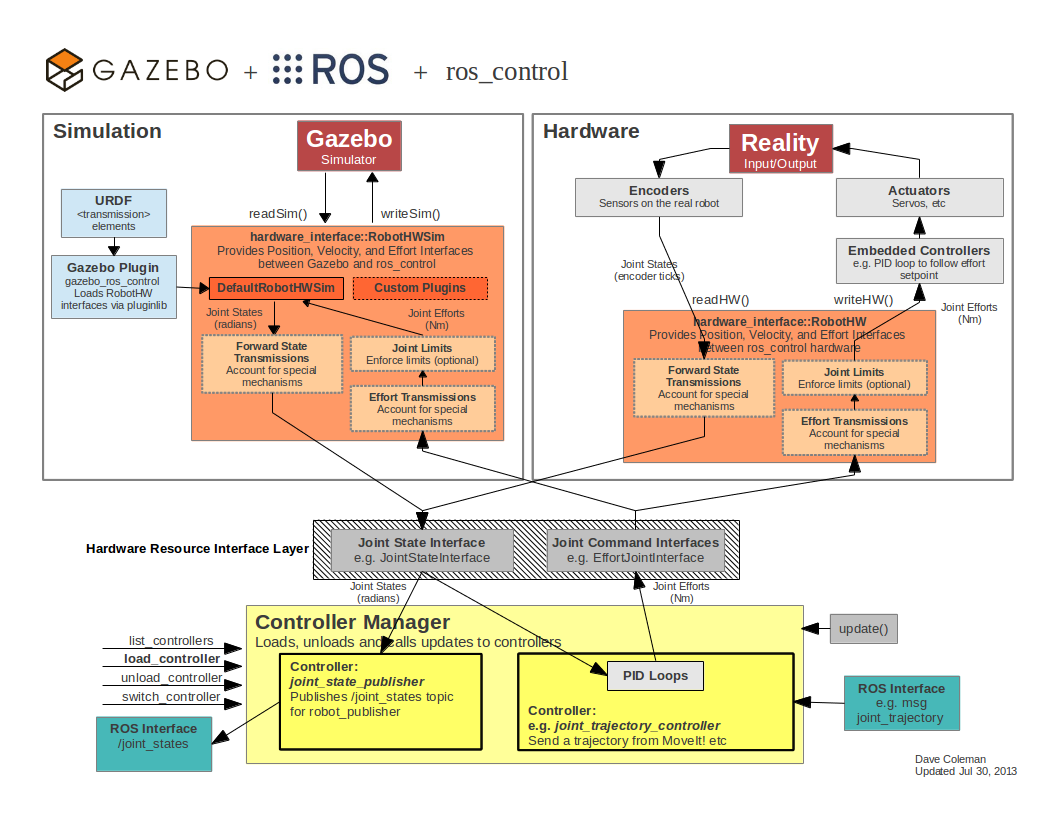
\includegraphics[width=\textwidth]{figures/ros_control_gazebo.png} 
	%Se que no te gusta, gordo, pero no la he encontrado en mejor calidad y son las 6 am
	\caption{ROS Control and Gazebo data flow}
	\label{fig:ros_control_gazebo}
\end{figure}

This architecture is meant to handle in real-time all the intermediary steps between the generation of joint commands for the robot by the custom controllers and their use in the platform, as well as for the feedback information flow in the opposite direction.
The idea behind it is that for most of the actuator and sensor types in a robot joint, the basic commands and readings can be abstracted to a few kinds, being currently implemented position, velocity and effort instances.
ROS control offers a set of controllers and transmissions for dealing with their transfer through the Hardware Resource Interface Layer, the Control Manager and the Controller modules in Figure \ref{fig:ros_control_gazebo}.
That leaves the "hardware interface" modules as the only part that needs to be defined by the user since they are platform dependent.
The interface with the real robot is discussed in \ref{sub:ros_control_hardware_locokit_interface}, while the one with the simulation is introduced in \ref{cha:simulation}.


% subsection ros_control (end)